\documentclass[twocolumn,a4j]{jsarticle}
\setlength{\topmargin}{-20.4cm}
\setlength{\oddsidemargin}{-10.4mm}
\setlength{\evensidemargin}{-10.4mm}
\setlength{\textwidth}{18cm}
\setlength{\textheight}{26cm}

\usepackage[top=15truemm,bottom=25truemm,left=15truemm,right=15truemm]{geometry}
\usepackage[latin1]{inputenc}
\usepackage{amsmath}
\usepackage{amsfonts}
\usepackage{amssymb}
\usepackage[dvipdfmx]{graphicx}
\usepackage[dvipdfmx]{color}
\usepackage{listings}
\usepackage{listings,jvlisting}
\usepackage{geometry}
\usepackage{framed}
\usepackage{color}
\usepackage[dvipdfmx]{hyperref}
\usepackage{ascmac}
\usepackage{enumerate}
\usepackage{tabularx}
\usepackage{cancel}
\usepackage{scalefnt}

\renewcommand{\figurename}{Fig.}
\renewcommand{\tablename}{Table }

\lstset{
basicstyle={\ttfamily},
identifierstyle={\small},
commentstyle={\smallitshape},
keywordstyle={\small\bfseries},
ndkeywordstyle={\small},
stringstyle={\small\ttfamily},
frame={tb},
breaklines=true,
columns=[l]{fullflexible},
xrightmargin=0zw,
xleftmargin=3zw,
numberstyle={\scriptsize},
stepnumber=1,
numbersep=1zw,
lineskip=-0.5ex
}

\makeatletter
\def\@maketitle
{
\begin{center}
{\LARGE \@title \par}
\end{center}
\begin{flushright}
{\large 報告書 NO.08 - 4\quad\@date\quad\@author}
\end{flushright}
\par\vskip 1.5em
}
\makeatother

\setcounter{tocdepth}{3}

\author{来代 勝胤}
\title{令和3年度 12月 第4週 報告書}
\date{2021/12/23}

\begin{document}
\columnseprule=0.1mm

\maketitle
\section*{報告内容}
\begin{enumerate}[1.]
    \item 進捗状況
    \item 再実験の実施
    \item 理論値の算出
    \item FFTの適用
    \item 位相角の算出
\end{enumerate}

\section{進捗状況}
今週は,測定したデータ処理を行うプログラムの作成を行った.
また,FFTを適用し位相角を求めるため,再度実験を行い
そのデータと理論値との差異を算出した.

\section{再実験の実施}
FFTを用いるためにデータ数を2の乗数に合わせなければならないことから,
前回行った実験と同様の手法で再実験を行うこととした.
今回は,22.5度刻みの計16方向からひずみセンサおよびロードセルの出力電圧の測定を行った.
実験結果を以下のTable 1および,Fig.1,Fig.2に示す.\\

\begin{table}[htbp]
    \begin{center}
        \caption{Result summary}
        \begin{tabular}{|p{20mm}|p{20mm}|p{20mm}|p{20mm}|}
            \hline
            \multicolumn{1}{|c|}{\textgt{Angle [deg]}} & \multicolumn{1}{|c|}{\textgt{Drag [V/V]}} & \multicolumn{1}{|c|}{\textgt{Lift [V/V]}} & \multicolumn{1}{|c|}{\textgt{Net [V/V]}} \\ \hline
            \multicolumn{1}{|c|}{0.0}                  & \multicolumn{1}{|r|}{-0.629891}           & \multicolumn{1}{|r|}{\textgt{0.096225}}   & \multicolumn{1}{|r|}{\textgt{0.637198}}  \\ \hline
            \multicolumn{1}{|c|}{22.5}                 & \multicolumn{1}{|r|}{-0.631390}           & \multicolumn{1}{|r|}{\textgt{-0.135281}}  & \multicolumn{1}{|r|}{\textgt{0.645720}}  \\ \hline
            \multicolumn{1}{|c|}{45.0}                 & \multicolumn{1}{|r|}{-0.505268}           & \multicolumn{1}{|r|}{\textgt{-0.400433}}  & \multicolumn{1}{|r|}{\textgt{0.644703}}  \\ \hline
            \multicolumn{1}{|c|}{67.5}                 & \multicolumn{1}{|r|}{-0.305154}           & \multicolumn{1}{|r|}{\textgt{-0.564455}}  & \multicolumn{1}{|r|}{\textgt{0.641660}}  \\ \hline
            \multicolumn{1}{|c|}{90.0}                 & \multicolumn{1}{|r|}{-0.065062}           & \multicolumn{1}{|r|}{\textgt{-0.626712}}  & \multicolumn{1}{|r|}{\textgt{0.630080}}  \\ \hline
            \multicolumn{1}{|c|}{112.5}                & \multicolumn{1}{|r|}{0.200668}            & \multicolumn{1}{|r|}{\textgt{-0.613089}}  & \multicolumn{1}{|r|}{\textgt{0.645094}}  \\ \hline
            \multicolumn{1}{|c|}{135.0}                & \multicolumn{1}{|r|}{0.368146}            & \multicolumn{1}{|r|}{\textgt{-0.531723}}  & \multicolumn{1}{|r|}{\textgt{0.646731}}  \\ \hline
            \multicolumn{1}{|c|}{157.5}                & \multicolumn{1}{|r|}{0.575943}            & \multicolumn{1}{|r|}{\textgt{-0.321693}}  & \multicolumn{1}{|r|}{\textgt{0.659694}}  \\ \hline
            \multicolumn{1}{|c|}{180.0}                & \multicolumn{1}{|r|}{0.632274}            & \multicolumn{1}{|r|}{\textgt{-0.079331}}  & \multicolumn{1}{|r|}{\textgt{0.637231}}  \\ \hline
            \multicolumn{1}{|c|}{202.5}                & \multicolumn{1}{|r|}{0.613635}            & \multicolumn{1}{|r|}{\textgt{0.171695}}   & \multicolumn{1}{|r|}{\textgt{0.637203}}  \\ \hline
            \multicolumn{1}{|c|}{225.0}                & \multicolumn{1}{|r|}{0.539625}            & \multicolumn{1}{|r|}{\textgt{0.364962}}   & \multicolumn{1}{|r|}{\textgt{0.651454}}  \\ \hline
            \multicolumn{1}{|c|}{247.5}                & \multicolumn{1}{|r|}{0.319874}            & \multicolumn{1}{|r|}{\textgt{0.550715}}   & \multicolumn{1}{|r|}{\textgt{0.636873}}  \\ \hline
            \multicolumn{1}{|c|}{270.0}                & \multicolumn{1}{|r|}{0.053645}            & \multicolumn{1}{|r|}{\textgt{0.634929}}   & \multicolumn{1}{|r|}{\textgt{0.637191}}  \\ \hline
            \multicolumn{1}{|c|}{292.5}                & \multicolumn{1}{|r|}{-0.179625}           & \multicolumn{1}{|r|}{\textgt{0.619397}}   & \multicolumn{1}{|r|}{\textgt{0.644917}}  \\ \hline
            \multicolumn{1}{|c|}{315.0}                & \multicolumn{1}{|r|}{-0.407471}           & \multicolumn{1}{|r|}{\textgt{0.503615}}   & \multicolumn{1}{|r|}{\textgt{0.647812}}  \\ \hline
            \multicolumn{1}{|c|}{337.5}                & \multicolumn{1}{|r|}{-0.575843}           & \multicolumn{1}{|r|}{\textgt{0.304549}}   & \multicolumn{1}{|r|}{\textgt{0.651418}}  \\ \hline
            \multicolumn{1}{|c|}{Average}              & \multicolumn{1}{|r|}{0.000257}            & \multicolumn{1}{|r|}{\textgt{-0.001664}}  & \multicolumn{1}{|r|}{\textgt{0.643436}}  \\ \hline
        \end{tabular}
    \end{center}
\end{table}

\newpage

\begin{figure}[htbp]
    \footnotesize
    \begin{center}
        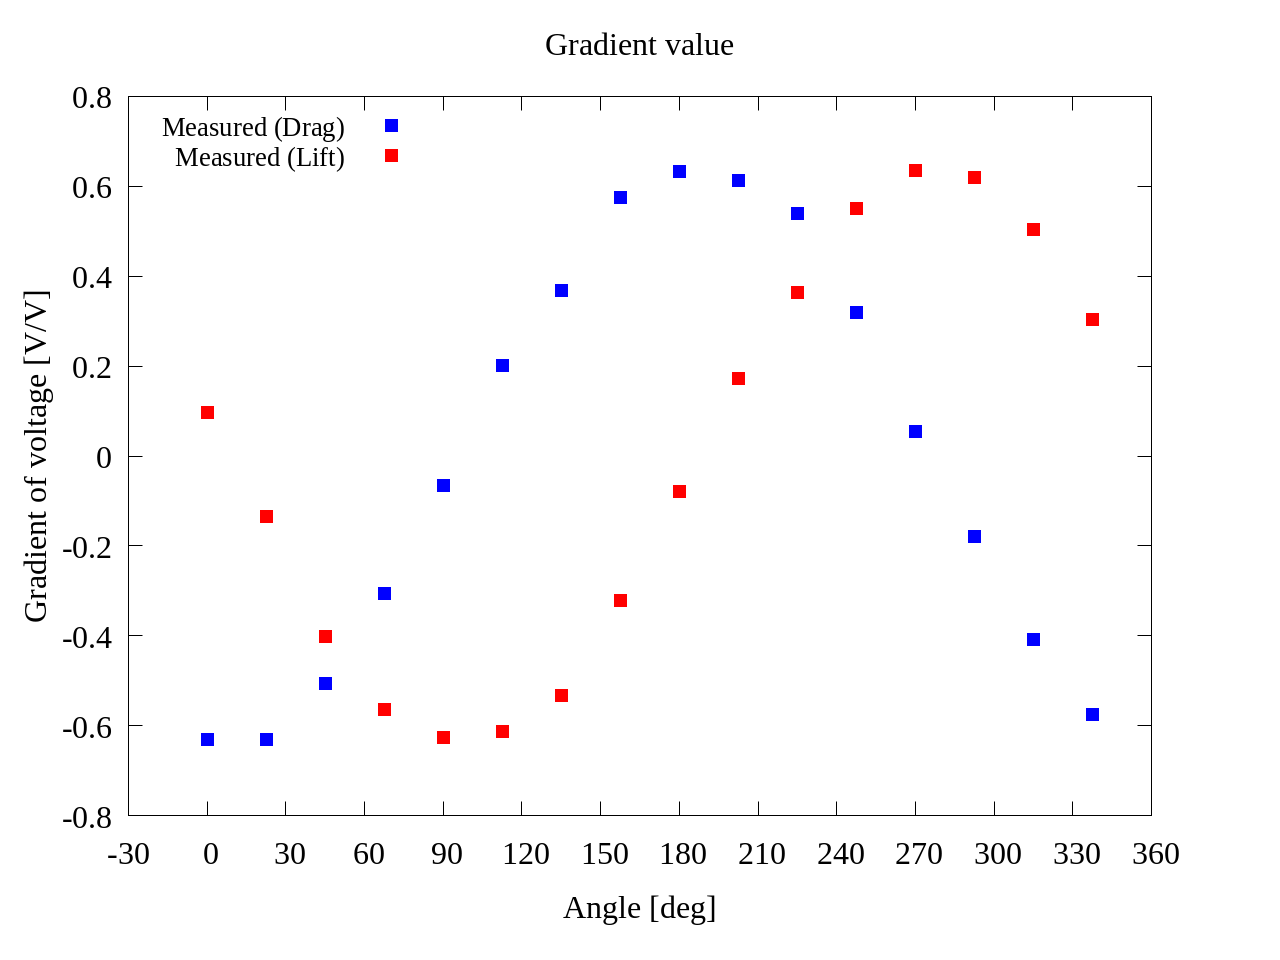
\includegraphics[width=88mm]{../images_2/05/05_summary-wave.png}
        \caption{Summary of gradient value}
        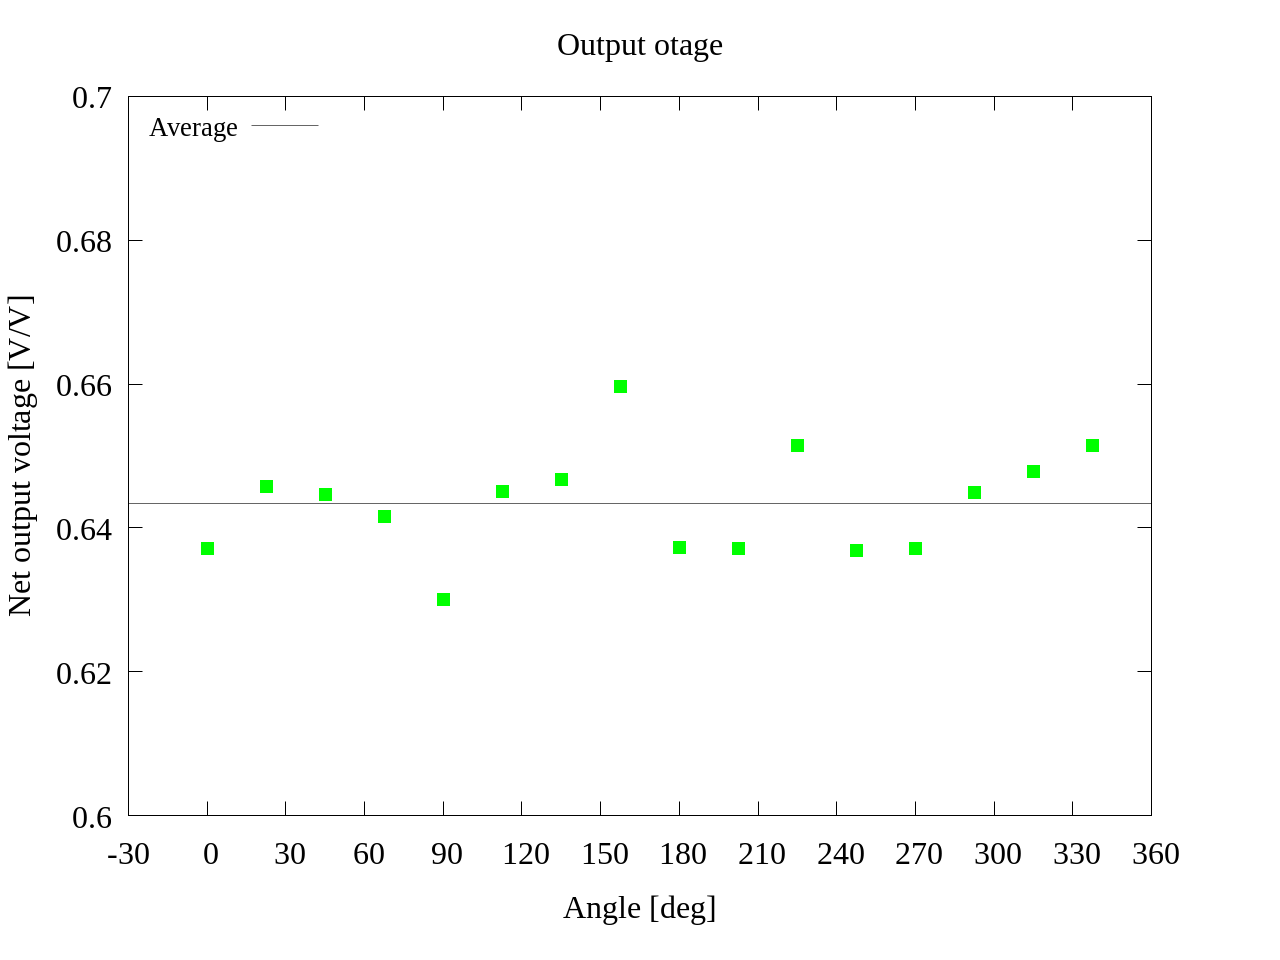
\includegraphics[width=88mm]{../images_2/05/05_summary-outputvoltage.png}
        \caption{Summary of net voltage value}
    \end{center}
\end{figure}

実験結果から算出した正味出力電圧の分散及び標準偏差を以下のTable 2 に示す.

\begin{table}[htbp]
    \begin{center}
        \caption{}
        \begin{tabular}{|p{20mm}|p{20mm}|}
            \hline
            \multicolumn{1}{|c|}{\textgt{分散}}     & \multicolumn{1}{|c|}{0.000051} \\ \hline
            \multicolumn{1}{|c|}{\textgt{標準偏差}} & \multicolumn{1}{|c|}{0.007133} \\ \hline
        \end{tabular}
    \end{center}
\end{table}

\newpage

\section{理論値の算出}
電圧の測定実験において,抗力および揚力の出力電圧は正弦波の位相がそれぞれ$-\pi/2$,$\pi$だけ
進んだ波形になると考えられる.

\begin{eqnarray*}
    \mathrm{Drag\;voltage} &=& A \sin\left(\omega t - \frac{\pi}{2}\right)\\
    \mathrm{Lift\;voltage} &=& A \sin\left(\omega t + \pi\right)\\
\end{eqnarray*}

ここで,Table 1の正味の出力電圧の平均値を振幅とし,
抗力および揚力についてそれぞれ位相が進んだ正弦波を作成した.
その算出結果と実験結果を重ねた図を以下のFig.3に示す.

\begin{figure}[htbp]
    \footnotesize
    \begin{center}
        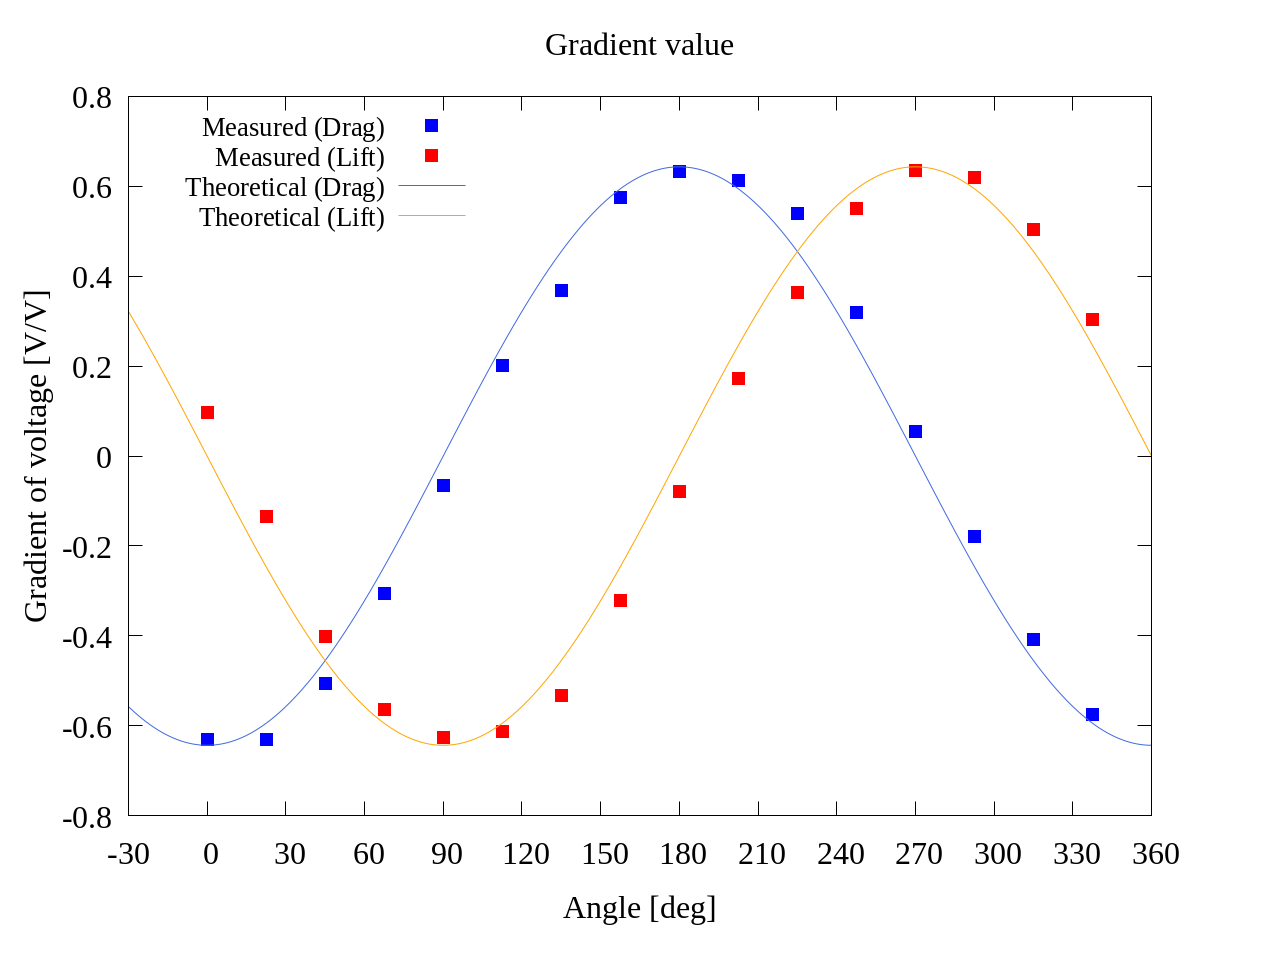
\includegraphics[width=88mm]{../images_2/20/20_adjust-value.png}
        \caption{value}
    \end{center}
\end{figure}

Fig.3をみると,実験結果は理論値に比べて抗力・揚力ともに
位相が遅れていることがわかる.
ここで,この結果から理論値との位相差を算出することを
目的としてデータの処理を行うこととした.

\section{FFTの適用}

測定した16点のデータを用いて,実験結果及び理論値について
FFTを適用した.その結果を以下のFig.4,Fig.5に示す.
また,Table 3にFFTを適用した結果のうち,波数1についての結果を以下に示す.

\newpage

\begin{figure}[htbp]
    \footnotesize
    \begin{center}
        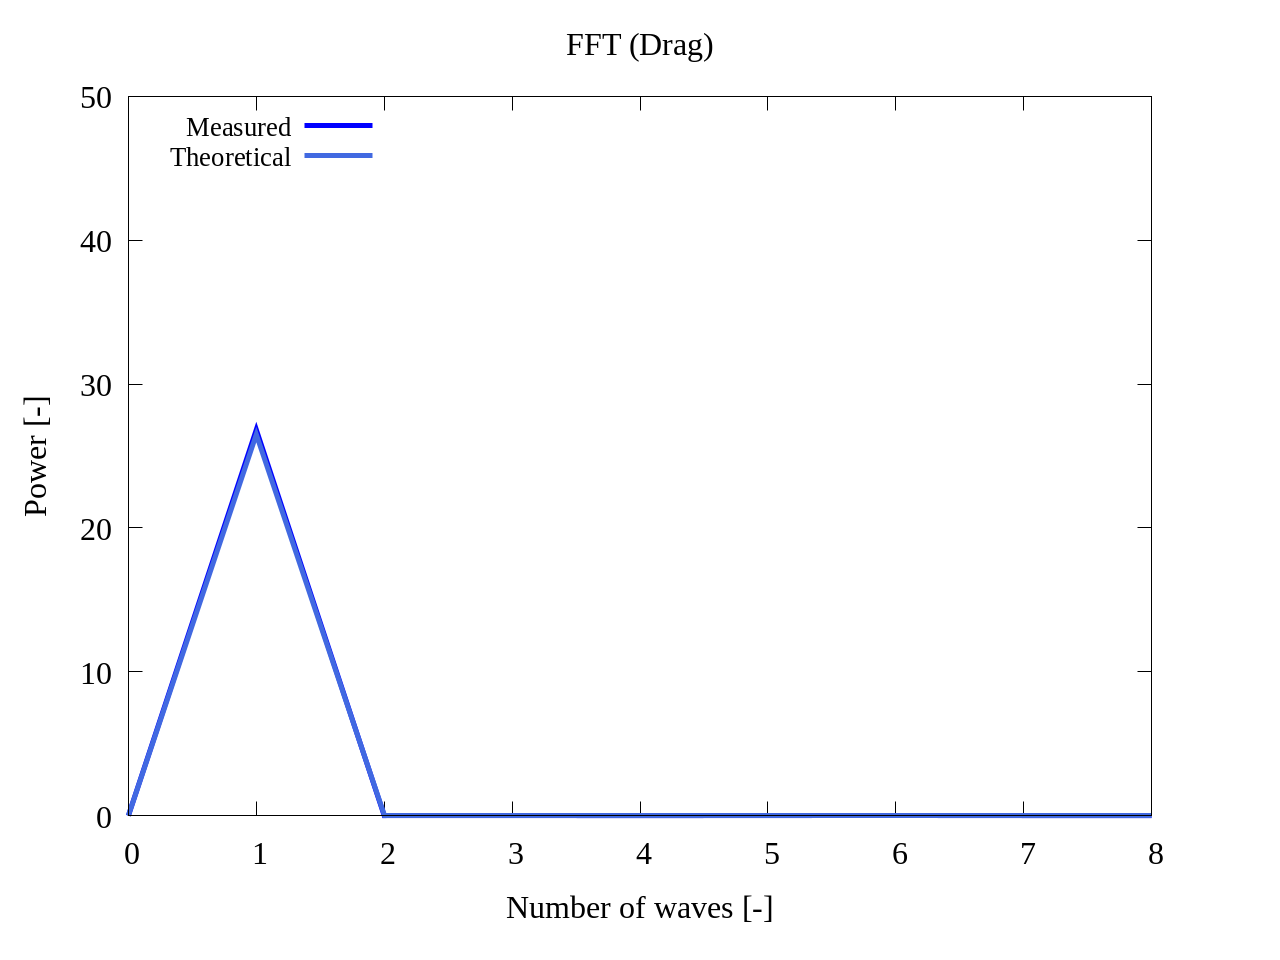
\includegraphics[width=88mm]{../images_2/27/27-3_fft-drag_summary.png}
        \caption{FFT Result [Drag]}
        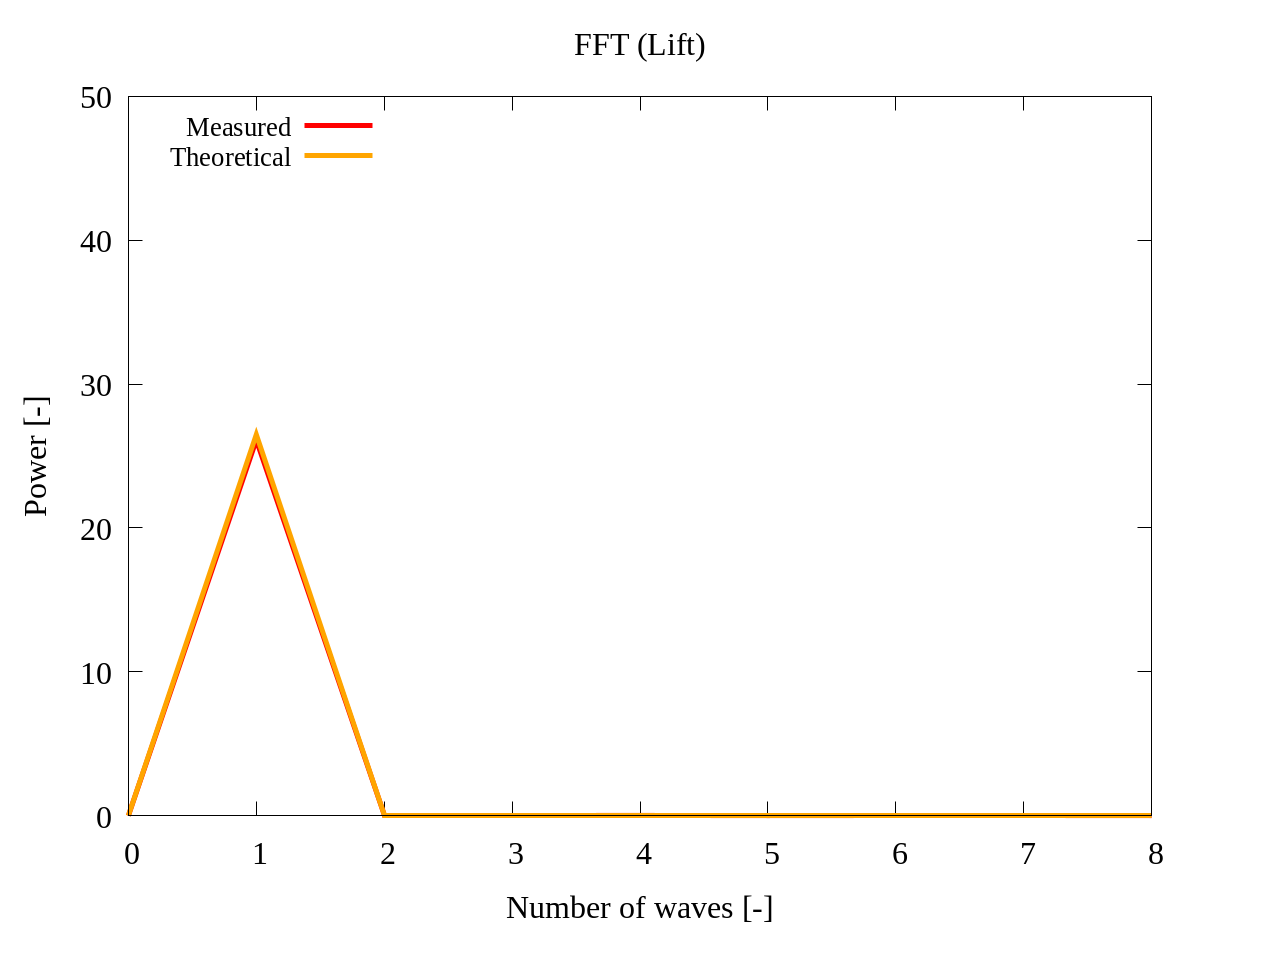
\includegraphics[width=88mm]{../images_2/27/27-4_fft-lift_summary.png}
        \caption{FFT Result [Lift]}
    \end{center}
\end{figure}

\begin{table}[htbp]
    \begin{center}
        \caption{FFT result}
        \begin{tabular}{|p{20mm}|p{20mm}|p{20mm}|p{20mm}|}
            \hline
            \multicolumn{1}{|c|}{}                 & \multicolumn{1}{|c|}{\textgt{Re}} & \multicolumn{1}{|c|}{\textgt{Im}}       & \multicolumn{1}{|c|}{\textgt{Power}}     \\ \hline
            \multicolumn{1}{|c|}{Measured [Drag]}  & \multicolumn{1}{|r|}{-5.148544}   & \multicolumn{1}{|r|}{\textgt{0.570901}} & \multicolumn{1}{|r|}{\textgt{26.833436}} \\ \hline
            \multicolumn{1}{|c|}{Measured [Lift]}  & \multicolumn{1}{|r|}{0.706293}    & \multicolumn{1}{|r|}{\textgt{5.061030}} & \multicolumn{1}{|r|}{\textgt{26.112873}} \\ \hline
            \multicolumn{1}{|c|}{Theorical [Drag]} & \multicolumn{1}{|r|}{-5.147490}   & \multicolumn{1}{|r|}{\textgt{0.000000}} & \multicolumn{1}{|r|}{\textgt{26.496654}} \\ \hline
            \multicolumn{1}{|c|}{Theorical [Lift]} & \multicolumn{1}{|r|}{0.000000}    & \multicolumn{1}{|r|}{\textgt{5.147490}} & \multicolumn{1}{|r|}{\textgt{26.496654}} \\ \hline
        \end{tabular}
    \end{center}
\end{table}

Fig.4,Fig.5をみると,実験結果と理論値のピークは一致していることがわかる.
また,Table 3をみると,パワースペクトル値は4つの条件に関しておおよそ一致していることがわかる.
したがって,FFTによって波の特徴を正しく捉えられており,抗力側及び揚力側に取り付けられているひずみセンサに
大きな個体差はないと考えられる.

\newpage

\section{位相角の算出}
ここで,Table 3の結果から以下の式をもとに位相角 $\varphi$ を算出した.
また,その結果を以下のTable 4に示す.

\begin{eqnarray*}
    \mathrm{\varphi \; [degree]} = \arctan \left(\frac{Im}{Re}\right) × \frac{180}{\pi}
\end{eqnarray*}

\begin{itemize}
    \item [※] ここでの位相角$\varphi$は,FFTの性質上,余弦波に対する位相角を示している.
\end{itemize}

\begin{table}[htbp]
    \begin{center}
        \caption{Phase angle}
        \begin{tabular}{|p{20mm}|p{20mm}|p{20mm}|}
            \hline
            \multicolumn{1}{|c|}{}                    & \multicolumn{1}{|c|}{\textgt{Drag [deg]}} & \multicolumn{1}{|c|}{\textgt{Lift [deg]}} \\ \hline
            \multicolumn{1}{|c|}{\textgt{Measured}}   & \multicolumn{1}{|r|}{-6.327446}           & \multicolumn{1}{|r|}{82.055387}           \\ \hline
            \multicolumn{1}{|c|}{\textgt{Theorical}}  & \multicolumn{1}{|r|}{0.000000}            & \multicolumn{1}{|r|}{90.000000}           \\ \hline
            \multicolumn{1}{|c|}{\textgt{Difference}} & \multicolumn{1}{|r|}{-6.327446}           & \multicolumn{1}{|r|}{-7.944613}           \\ \hline
        \end{tabular}
    \end{center}
\end{table}

Table 4をみると,抗力及び揚力方向に対して,
ひずみセンサの取付角度に小さな差異が存在する可能性が考えられる.

\end{document}